%%%%%%%%%%%%%%%%%%%%%%%%%%%%%%%%%%%%%%%%%
% Short Sectioned Assignment LaTeX Template Version 1.0 (5/5/12)
% This template has been downloaded from: http://www.LaTeXTemplates.com
% Original author:  Frits Wenneker (http://www.howtotex.com)
% License: CC BY-NC-SA 3.0 (http://creativecommons.org/licenses/by-nc-sa/3.0/)
%%%%%%%%%%%%%%%%%%%%%%%%%%%%%%%%%%%%%%%%%

%----------------------------------------------------------------------------------------
%	PACKAGES AND OTHER DOCUMENT CONFIGURATIONS
%----------------------------------------------------------------------------------------

\documentclass[paper=a4, fontsize=10pt]{scrartcl} % A4 paper and 11pt font size

% ---- Entrada y salida de texto -----

\usepackage[T1]{fontenc} % Use 8-bit encoding that has 256 glyphs
\usepackage[utf8]{inputenc}
%\usepackage{fourier} % Use the Adobe Utopia font for the document - comment this line to return to the LaTeX default

% ---- Idioma --------

\usepackage[spanish, es-tabla]{babel} % Selecciona el español para palabras introducidas automáticamente, p.ej. "septiembre" en la fecha y especifica que se use la palabra Tabla en vez de Cuadro

% ---- Otros paquetes ----

\usepackage{amsmath,amsfonts,amsthm} % Math packages
%\usepackage{graphics,graphicx, floatrow} %para incluir imágenes y notas en las imágenes
\usepackage{graphics,graphicx, float, url} %para incluir imágenes y colocarlas

% Para hacer tablas comlejas
%\usepackage{multirow}
%\usepackage{threeparttable}

%\usepackage{sectsty} % Allows customizing section commands
%\allsectionsfont{\centering \normalfont\scshape} % Make all sections centered, the default font and small caps

\usepackage{fancyhdr} % Custom headers and footers
\pagestyle{fancyplain} % Makes all pages in the document conform to the custom headers and footers
\fancyhead{} % No page header - if you want one, create it in the same way as the footers below
\fancyfoot[L]{} % Empty left footer
\fancyfoot[C]{} % Empty center footer
\fancyfoot[R]{\thepage} % Page numbering for right footer
\renewcommand{\headrulewidth}{0pt} % Remove header underlines
\renewcommand{\footrulewidth}{0pt} % Remove footer underlines
\setlength{\headheight}{13.6pt} % Customize the height of the header

\numberwithin{equation}{section} % Number equations within sections (i.e. 1.1, 1.2, 2.1, 2.2 instead of 1, 2, 3, 4)
\numberwithin{figure}{section} % Number figures within sections (i.e. 1.1, 1.2, 2.1, 2.2 instead of 1, 2, 3, 4)
\numberwithin{table}{section} % Number tables within sections (i.e. 1.1, 1.2, 2.1, 2.2 instead of 1, 2, 3, 4)

\setlength\parindent{0pt} % Removes all indentation from paragraphs - comment this line for an assignment with lots of text

\newcommand{\horrule}[1]{\rule{\linewidth}{#1}} % Create horizontal rule command with 1 argument of height


% ---- Otros paquetes --------

\usepackage{enumerate}
\usepackage{subfig} % Múltiples figuras juntas
\usepackage{multirow} % Tablas
%\usepackage{xcolor}
\usepackage[table]{xcolor}
\usepackage{slashbox} % Barra separadora tablas

\usepackage{anysize}
\marginsize{2.5cm}{2.5cm}{2cm}{2cm} %izq, derecha, arriba

\usepackage[colorlinks=true, citecolor=red, urlcolor=blue]{hyperref}

%----------------------------------------------------------------------------------------
%	TÍTULO Y DATOS DEL ALUMNO
%----------------------------------------------------------------------------------------

\title{
\normalfont \normalsize
\textsc{{\bfseries Inteligencia Computacional (2018-2019)} \\
			Ciencias de la Computación e Inteligencia Artificial\\[0.5cm]
			Máster Profesional en Ingeniería Informática\\ Universidad de Granada}
			\\ [25pt] % Your university, school and/or department name(s)
\horrule{0.5pt} \\[0.4cm] % Thin top horizontal rule
\bfseries \huge Práctica de algoritmos evolutivos \\% The assignment title
\Large Problemas de optimización combinatoria - QAP\\
%\huge Aplicación para la gestión de ángulos articulares %
\horrule{2pt} \\[0.5cm] % Thick bottom horizontal rule
}

\author{Mª del Mar Alguacil Camarero} % Nombre y apellidos

\date{} % Incluye la fecha actual

%----------------------------------------------------------------------------------------
% DOCUMENTO
%----------------------------------------------------------------------------------------

\begin{document}

\maketitle % Muestra el Título

\newpage %inserta un salto de página

\tableofcontents % para generar el índice de contenidos

%\listoffigures

%\listoftables

\newpage

%\begin{enumerate}[\quad 1)]

%----------------------------------------------------------------------------------------
%	INTRODUCCIÓN
%----------------------------------------------------------------------------------------
\section{Introducción}

El Problema de la Asignación Cuadrática (QAP) está considerado como uno de los problemas de optimización combinatoria más complejos, siendo NP-completo, es decir, la resolución de incluso problemas pequeños de tamaño n>25 se considera una tarea computacional muy costosa.\\

El problema general consiste en encontrar la asignación óptima de $n$ unidades a $n$ localizaciones, conociendo la distancia entre las primeras y el flujo existente entre las segundas. Formalmente, sean $n$ unidades y $n$ localizaciones, si denotamos $d(i,j)$ a la distancia de la localización $i$ a la $j$ y $w(i,j)$ al peso asociado al flujo que circula entre la unidad $i$ y la $j$, hemos de encontrar la asignación de instalaciones a localizaciones que minimice la función de coste

$$
	\sum_{i,j=1}^n w(i,j) d(p(i), p(j))
$$
donde $p(\cdot)$ define la permutación sobre el conjunto de instalaciones.\\

El problema de la asignación cuadrática es un problema habitual en Investigación Operativa y, además de utilizarse para decidir la ubicación de plantas de producción, también se puede utilizar como modelo para colocar los componentes electrónicos de un circuito sobre una placa impresa o los módulos de un circuito integrado en la superficie de un microchip.\\

Por su interés teórico y práctico, existe una variedad muy amplia de algoritmos que abordan la resolución del problema de la asignación cuadrática. Al ser un problema NP-completo, el diseño y aplicación de algoritmos exactos para su resolución no es viable cuando $n$ es grande. Nos centraremos, por tanto, en el diseño de algoritmos evolutivos y evaluaremos su rendimiento sobre instancias concretas del problema.

%----------------------------------------------------------------------------------------
%	IMPLEMENTACIÓN
%----------------------------------------------------------------------------------------
\section{Implementación}

En esta sección se explicarán las distintas variantes que se han realizado de los algoritmos genéticos para resolver el problema de la asignación cuadrática de forma viable.

\subsection{Algoritmo genético estándar}

\begin{itemize}
	\item \textbf{\textit{Generación de la población inicial:}} Las soluciones iniciales se generan de forma \textbf{aleatoria}.
	
	\item \textbf{\textit{Esquema de evolución:}} Se seleccionan únicamente \textbf{dos padres} para realizar las distintas etapas de cruce, mutación y reemplazamiento.
	
	\item \textbf{\textit{Operador de selección:}}
	\begin{itemize}
		\item \textbf{Torneo n-ario:} consiste en elegir aleatoriamente $n$ individuos distintos de la población y seleccionar el mejor de ellos. Dicho torneo se aplicará dos veces para elegir los dos padres que serán posteriormente recombinados (cruzados).
		\item \textbf{Regla de la ruleta:} los padres se seleccionan de acuerdo a su \textit{fitness}. Por lo tanto, los mejores individuos son los que tienen mayores posibilidades de ser elegidos. 
		\item \textbf{Aleatorios:} se eligen dos padres distintos de forma totalmente aleatoria.
	\end{itemize}
	
	\item \textbf{\textit{Operador de cruce:}} se emplea el \textbf{operador de cruce PMX} consistente en elegir una subcadena aleatoria y establecer una correspondencia por posición entre las asignaciones contenidas en ellas. Cada hijo contiene la subcadena seleccionada de uno de los padres y el mayor número posible de asignaciones en las posiciones definidas por el otro padre. Cuando se forma un ciclo, se sigue la correspondencia fijada para incluir la asignación nueva. En este caso, suponemos que la probabilidad de cruce es uno, es decir, siempre se cruzan.
	
	\item \textbf{\textit{Operador de mutación:}} se emplea el \textbf{operador de intercambio} donde se seleccionan dos alelos aleatoriamente y se intercambian. Cabe notar que existe una probabilidad de mutación por cromosoma y por gen que se tendrá en cuenta para realizar los diferentes experimentos.
	
	\item \textbf{\textit{Esquema de reemplazamiento:}} Los pasos explicados anteriormente se aplican hasta rellenar una nueva generación y la población de hijos sustituirá automáticamente a la actual, pero conservando la mejor solución si tiene un mayor coste que la peor de la nueva población.
\end{itemize}

Todo este proceso se realizará según un número de épocas prefijado.
	
\subsection{Algoritmo memético}

Para problemas NP, los algoritmos greedy no propocionan soluciones óptimas, pero pueden sernos útiles como técnicas de optimización local para obtener soluciones aceptables de forma muy eficiente.\\

En busca de obtener mejores resultados se utiliza un estrategia de trasposición donde se comienza con una permutación inicial y se va intercambiando las posiciones de dos instalaciones. En este caso se ha implementado el algoritmo greedy basado en 2-opt donde se realizan $n(n-1)/2$ intercambios antes de modificar la mejor solución actual S y, en cada iteración, se realiza un único intercambio (aquel con el que se obteng un coste menor de entre todas las trasposiciones). \\

Este algoritmo se utiliza para dotar de capacidad de "aprendizaje" a los individuos de la población.

\begin{itemize}
	\item \textbf{Variante \textit{baldwidiana}:} para evaluar el \textit{fitness} de cada individuo se utiliza dicho individuo como punto de partida para realizar una búsqueda local hasta alcanzar un óptimo local y se utiliza el valor de dicho óptimo para determinar el \textit{fitness} del individuo. Sin embargo, a la hora de formar descendientes, se utiliza el material genético del individuo original (sin incluir las mejoras ``aprendidas'' al aplicar la técnica de búsqueda local).
	
	\item \textbf{Variante \textit{lamarckiana}:} el \textit{fitness} de los individuos se evalúa igual que en la variante \textbf{baldwidiana}, sin embargo, en este caso, los descendientes de un individuo se forman a partir de la solución mejorada que se consigue utilizando técnicas de búsqueda local (los descendientes heredan los rasgos adquiridos por sus padres en su proceso de ``aprendizaje'').
\end{itemize}

Además también se ha probado a utilizar dicho algoritmo (reemplazándolo o no) pero simplemente a la mejor solución encontrada intentando minimizar el tiempo de ejecució y consiguiendo mejoras con respecto al algoritmo genético estándar.

%----------------------------------------------------------------------------------------
%	RESULTADOS
%----------------------------------------------------------------------------------------
\section{Resultados}

En esta sección se mostrarán alguno de los resultados obtenidos durante la ejecución de los distintos algoritmos.\\

Inicialmente se comprobaron los algoritmos más rápidos para tener una visión general de las mejoras que se podrían producir aplicando las variantes \textit{lamarckiana} y \textit{baldwidiana}.

	\begin{figure}[H]
	\centering
	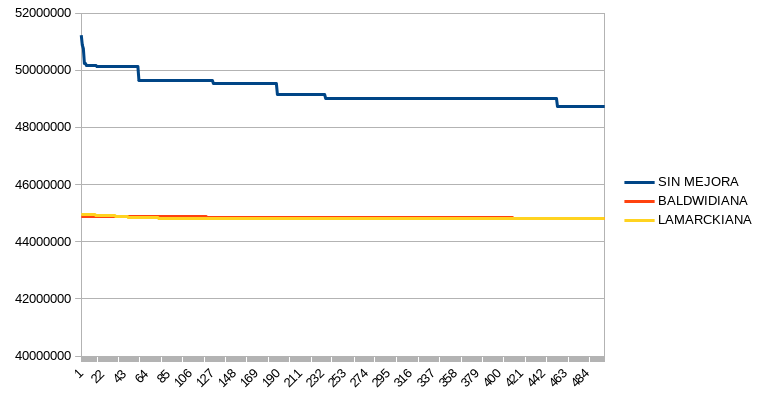
\includegraphics[scale=0.8]{images/AGEcomp.png} 
	\caption{Comparación de algoritmos rápidos.}
	\label{perc}
	\end{figure}
	
La diferencia obtenida con la búsqueda local en las mejores soluciones en comparación con el algoritmo estándar es notable, sin embargo, la diferencia entre estos no se puede apreciar en la imagen anterior por lo que se muestra a continuación.

	\begin{figure}[H]
	\centering
	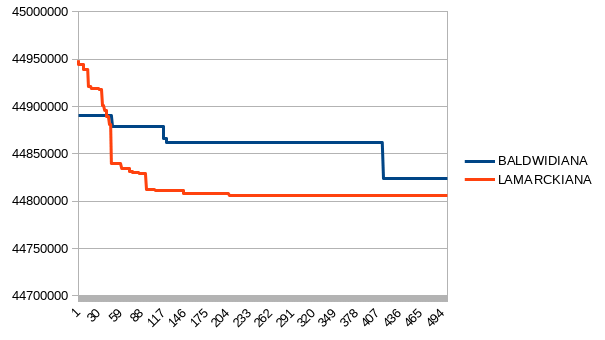
\includegraphics[scale=0.9]{images/AGEcompBL.png} 
	\caption{Comparación de las variantes simples y rápidas.}
	\label{perc}
	\end{figure}

Podemos observar que la variante \textit{lamarckiana} es mejor que la \textit{baldwidiana} por lo que la mayoria de mejoras se intentan realizar teniendo en cuenta esta.

\subsection{Ajustes de parámetros}

Inicialmente se probó poblaciones de 50, 100 y 150 para comprobar si metiéndole más variedad de individuos mejora el algoritmo sin embargo se comprobó que a partir de 100 no es notable ya que los individuos tienden a ser más parecidos por lo que simplemente iba a ralentizar la ejecución. En consecuencia, se decidió mantener a 100.\\

También la mutación es necesaria para tener mayor variedad en la población e intentar escapar de mínimos locales, pero mutar siempre puede provocar que no se explore a fondo un espacio donde podría haber una buena solución por lo que se prueban distintas probabilidades de mutación y mutación por gen.

	\begin{figure}[H]
	\centering
	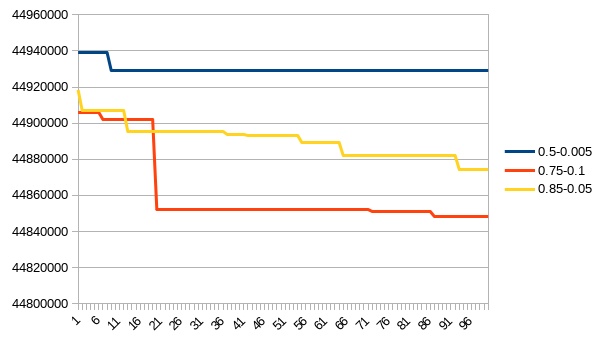
\includegraphics[scale=0.9]{images/Lamarck/AGEcompMUT.png} 
	\caption{Resultados variando las probabilidades de mutación.}
	\label{perc}
	\end{figure}
	
Pero se comprobó que la diferencia de resultados es más bien debida a la aleatoridad de las soluciones en los dos últimos que a dichas probabilidades por lo que en un principio se estableció en 0.75 y 0.05 la probabilidad de mutación y mutación por gen, respectivamente.\\

Además se dició verificar si el mecanismo de selección era relevante. 

	\begin{figure}[H]
	\centering
	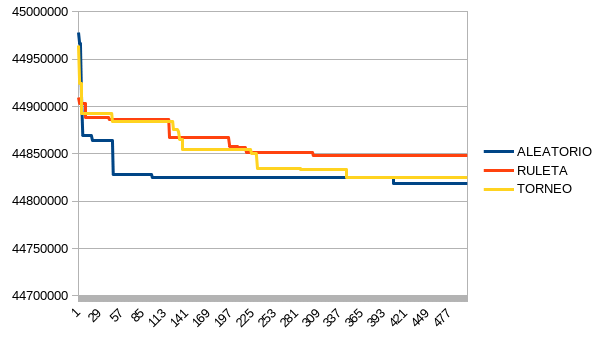
\includegraphics[scale=0.9]{images/Lamarck/AGE-ATR.png} 
	\caption{Comparación de mecanismos de selección en la variante \textit{lamarckiana}.}
	\label{perc}
	\end{figure}
	
	\begin{figure}[H]
	\centering
	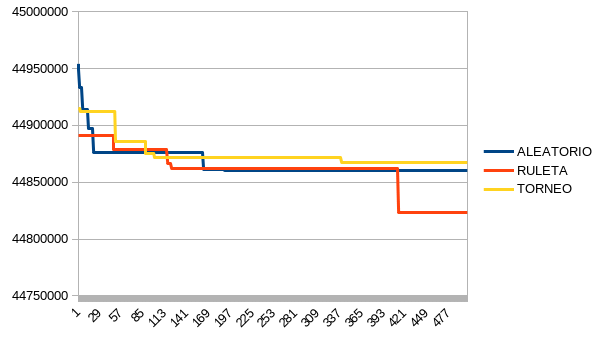
\includegraphics[scale=0.9]{images/AGE-BaldwidART.png} 
	\caption{Comparación de mecanismos de selección en la variante \textbf{baldwidiana}.}
	\label{perc}
	\end{figure}

Observando de nuevo que las diferentes eran más producidas por la aleatoridad asociada.\\

Por último, se decidió el número de individuos en el torneo, el cual debe ser bajo (en comparación con los individuos totaltes de la población) para permitir tener individuos no muy parecidos en esta. 

	\begin{figure}[H]
	\centering
	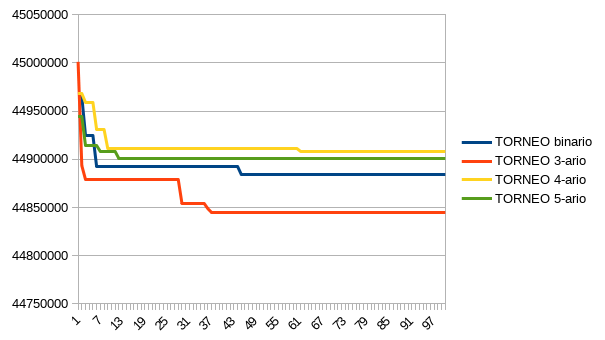
\includegraphics[scale=0.9]{images/Lamarck/AGE-TORNEO.png} 
	\caption{Comparación de mecanismos de selección en la variante \textit{lamarckiana}.}
	\label{perc}
	\end{figure}
	
Se puede observar que se obtienen individuos mejores al utilizar valores de $n$ igual a 2 y 3.

\subsection{Comparación de algoritmos}

Por último se muestra una tabla comparativa de los distintos resultados obtenidos así como sus tiempos:

	\begin{figure}[H]
	\centering
	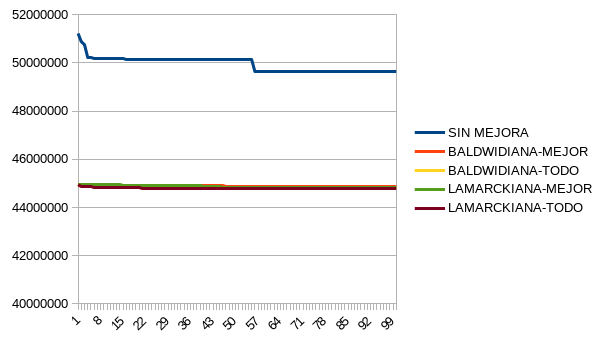
\includegraphics[scale=0.9]{images/AGcomp.png} 
	\caption{Comparación de los distintos métodos implementados.}
	\label{perc}
	\end{figure}
	
	\begin{figure}[H]
	\centering
	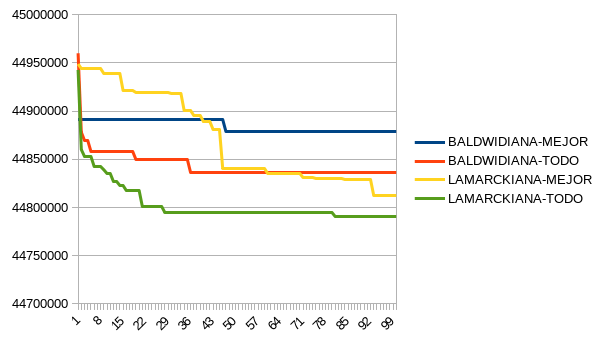
\includegraphics[scale=0.9]{images/AGcompBL.png} 
	\caption{Comparación de los distintos métodos implementados.}
	\label{perc}
	\end{figure}
	

\begin{table}[H]
\centering
\begin{tabular}{|l|c|}
\hline
                                     & \textbf{Tiempo (s)} \\ \hline
\textbf{General}                     & 0.645957            \\ \hline
\textbf{Variante \textit{baldwidiana} rápida} & 47.7497             \\ \hline
\textbf{Variante \textit{baldwidiana}}        & 2682.42             \\ \hline
\textbf{Variante \textit{lamarckiana} rápida} & 21.7687             \\ \hline
\textbf{Variante \textit{lamarckiana}}        & 2595.68             \\ \hline
\end{tabular}
\end{table}

Podemos observar, como era de esperarse, que los tiempos en las variantes donde se aplica la búsqueda local en cada individuo de la población son mucho más del doble. Sin embargo, las mejoras que se obtienen son casi inapreciales si tenemos en cuenta en esto. Por tanto, no podemos concluir que existe un método que sobresalga por completo pero podríamos decir que la mejor variante resultados/tiempo sería la variante \textit{lamarckiana} donde sólo se aplica optimización al mejor individuo perteneciente a la población de hijos aunque con el método donde se ha aplicado en toda la población se ha obtenido una mejor solución.\\

Cabe notar que también se comprobó aplicar búsqueda local cada 10 generaciones durante 500 épocas pero los resultados y tiempos que se obtuvieron fueron similares. Sin embargo, en una última prueba se decidió cambiar el número de integrantes en el torneo a 7 individuos y 1000 épocas (tardando 2976.31s), y sorprendentemente se obtuvieron mejores resultados, llegando a un coste de 44771590 en la iteración 431. 

\subsection{Resultado final}

El mejor resultado que se obtuvo fue con la variante \textit{lamarckiana}:

\begin{itemize}
	\item \textit{Tamaño de la población:} 100
	
	\item \textit{Número de épocas:} 1000
	
	\item \textit{Probabilidad de mutación por individuo:} 0.75
	
	\item \textit{Probabilidad de mutación por gen:} 0.05
	
	\item \textit{Operador de selección:} torneo 7-ario
	
\end{itemize}

\quad\\

Obteniendo la siguiente solución (cuyo \textit{fitness} asociado es 44771590):\\

0 254 171 112 186 134 101 156 104 176 216 211 218 126 63 141 34 222 131 231 144 71 149 13 22 74 197 241 99 151 129 64 239 166 250 69 180 43 67 228 39 89 116 168 37 41 190 123 188 26 248 7 111 28 119 193 121 108 49 220 153 31 158 19 82 175 146 4 163 226 91 208 46 205 86 97 138 32 94 214 252 9 77 52 183 60 56 245 178 201 2 235 184 27 244 42 96 185 225 162 217 210 58 209 221 164 62 105 78 107 20 73 155 1 55 238 16 57 38 167 177 132 170 100 137 18 187 76 98 54 103 61 172 128 95 33 117 30 40 66 79 113 247 240 36 219 160 135 251 242 48 83 21 215 75 24 142 93 44 59 195 182 192 196 14 50 133 122 29 206 173 232 181 72 51 223 106 154 102 90 118 234 115 127 88 136 3 130 237 47 169 159 140 199 212 35 202 213 253 204 198 114 174 230 249 12 23 236 227 109 179 8 110 152 5 92 150 6 87 124 243 143 81 10 25 68 80 157 189 65 45 191 11 120 165 147 17 70 207 229 255 15 203 233 224 194 139 148 246 53 200 145 85 84 161 125 

\section{Conclusiones}

Se ha realizado una implementación del algoritmo genético estándar además de las variantes \textit{baldwidiana} y \textit{lamarckiana} para resolver el problema la asignación cuadrática aplicado al conjunto de datos \texttt{tai256c}.\\

A continuación se realizó una comparación entre los distintos métodos observados, comprobando que efectivamente las variantes aplicadas al algoritmo genético general mejoraban la solución en un menor número de épocas, dando los mejores resultados las variantes \textit{lamarckianas}. \\

En busca de la mejor solución se intentó ajustar los distintos parámetros en la variante rápida pero en la mayoría de los casos no se conseguía mejoras notables. \\

Los métodos convergían rápidamente hacia distintos mínimos locales, lo que ha impedido encontrar la mejor solución conocida hasta el momento. Sin embargo, se ha conseguido obtener una permutación bastante cercana a esta, cuyo \textit{fitness} asociado ha sido de 44771590.

%----------------------------------------------------------------------------------------
%	REFERENCIAS
%----------------------------------------------------------------------------------------

\newpage

\bibliographystyle{plain} % hay varias formas de citar

\begin{thebibliography}{99} %Principio Bibliografía (99 max elementos)

	%\bibitem{virtual} Virtualización. (24 de septiembre de 2015):
	%\url{http://www.vmware.com/latam/virtualization/how-it-works}.

	\bibitem{ic} Material de la asignatura de Inteligencia Computacional\\
		\url{http://elvex.ugr.es/decsai/computational-intelligence/}
	
	\bibitem{mh} Material de la asignatura de Metaheurística\\
		\url{https://sci2s.ugr.es/graduateCourses/Metaheuristicas}
			
	%\bibitem{berzal} Berzal, Fernando. \textit{Redes neuronales \& Deep Learning}, 2018.
		
	
\end{thebibliography}

\end{document}
